\begin{exo}

Soit $E$ un ensemble convexe et compact et $f : E \rightarrow \mathbb { R }$ une fonction
 convexe  $\beta$-régulière, où $\beta$ est un paramètre connu. On considère l'algorithme
 \ref{fig:algo} ci-dessous, où $\gamma_s = \frac{2}{s}$, pour tout $s=1$ à $T$. Soit $D$ le diamètre
 de $E$.

\begin{figure}[H]
  \centering
  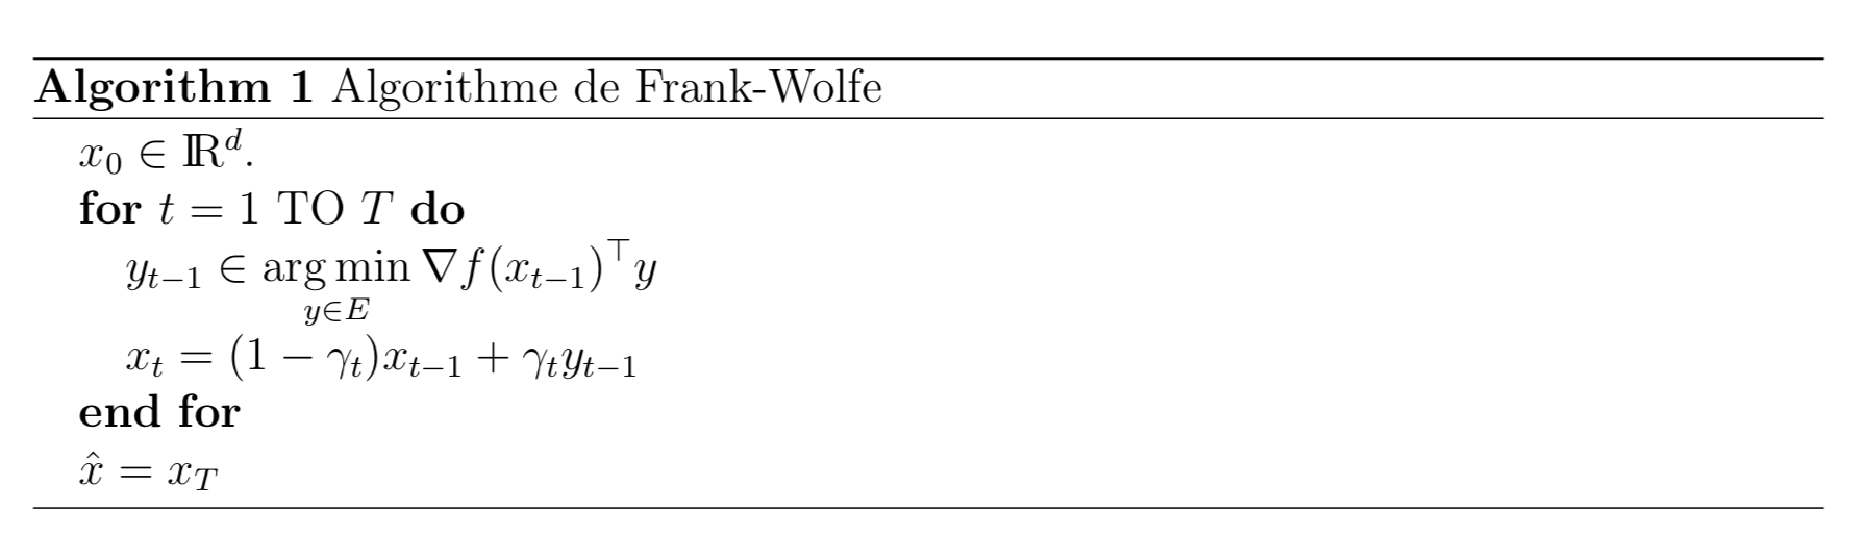
\includegraphics[scale=0.4]{algo}
  % \caption{}
  \label{fig:algo}
\end{figure}
\end{exo}

\begin{qst}

Montrer que :
\begin{align}
  \forall t \in \acc{1 \ldots T} \quad f \left( x _ { t } \right) - f \left( x _ { t - 1 } \right) \leq \gamma _ { t } \nabla f \left( x _ { t - 1 } \right) ^ { \top } \left( y _ { t - 1 } - x _ { t - 1 } \right) +\frac { \beta } { 2 } \gamma _ { t } ^ { 2 } D ^ { 2 }
\end{align}
\end{qst}


\begin{rep}


En appliquant la propriété de $\beta$-régularité aux points $x_{t-1}$ et $x_t$, puis la définition de $x_t$, on a successivement :
\begin{align*}
  f(x_{t})-f(x_{t-1}) &\leq \ps{\grad f(x_{t-1})}{x_t-x_{t-1}}+\frac{\beta}{2}
  \norme{x_t-x_{t-1}}^2\\
  &\leq \ps{\grad f(x_{t-1})}{\gamma_t\cdot (y_{t-1}-x_{t-1})}+\frac{\beta}{2}
  \norme{\gamma_t\cdot (y_{t-1}-x_{t-1})}^2
\end{align*}
Comme $y _ { t - 1 } \in \underset { y \in E } { \arg \min } \nabla f \left( x _ { t - 1 } \right) ^ { \top } y$ (qui existe bien car l'on optimise une fonction linéaire
 donc continue sur un compact), et que $E$ est fermé, ceci assure que $y_{t-1}\in E$.

 De plus, en utilisant la convexité de $E$, une récurrence immédiate montre que $x_{t-1}$
 appartient aussi à $E$.
 D'où
 \begin{align*}
\norme{y_{t-1}-x_{t-1}} \leq \sup_{(x,y)\in E} \norme{x-y} := D,
 \end{align*}
ce qui permet de conclure.
\end{rep}

\begin{qst}

On pose $\delta_t = f(x_t)-f(\xopt)$. En utilisant la définition de $y_{t-1}$, en
déduire que :
\begin{align} \label{eq:tele}
\delta _ { t } \leq \left( 1 - \gamma _ { t } \right) \delta _ { t - 1 } + \frac { \beta } { 2 } \gamma _ { t } ^ { 2 } D ^ { 2 }
\end{align}
\end{qst}

\begin{rep}

Utilisons l
a définition de $y_{t-1}$ comme suggéré. On a :
\begin{align*}
  \forall x \in E \quad   f(x_{t})-f(x_{t-1}) &\leq
  \gamma_t\cdot\ps{\grad f(x_{t-1})}{ y_{t-1}-x_{t-1}}+\frac{\beta \gamma_t^2}{2}
  D^2\\
  &\leq   \gamma_t\cdot\ps{\grad f(x_{t-1})}{ x-x_{t-1}}+\frac{\beta \gamma_t^2}{2}
    D^2\\
    \Leftrightarrow \forall x \in E \qquad \delta_t - \delta_{t-1} &\leq \gamma_t\cdot\ps{\grad f(x_{t-1})}{ x-x_{t-1}}+\frac{\beta \gamma_t^2}{2}
      D^2
\end{align*}

Pour quelle $x$ a-t-on : $\displaystyle \gamma_t \cdot  \ps{\grad f(x_{t-1})}{ x-x_{t-1}}
\leq - \gamma_t \cdot  \prt{f(x_t)-f(\xopt)}$ ?

Il suffit de prendre $x = \xopt$ puis d'appliquer la simple convexité de $f$ aux points
 $\xopt$ et $x_{t+1}$ pour en déduire le résultat.

\end{rep}

\begin{qst}

Conclure que $\displaystyle f ( \hat { x } ) - f \left( x ^ { * } \right) \leq \frac { \beta D ^ { 2 } } { T }$.
\end{qst}

\begin{rep}

En appliquant récursivement l'équation \eqref{eq:tele}, on a :
\begin{align*}
  f(x_T)-f(\xopt) = \delta_T &\leq \prt{1-\gamma_T}\delta_{T-1}+ \frac{\beta}{2} D^2 \gamma_T^2\\
&\leq \prt{1-\gamma_T}\acc{\prt{1-\gamma_{T-1}}\delta_{T-2}+ \frac{\beta}{2} D^2 \gamma_{T-1}^2}+ \frac{\beta}{2} D^2 \gamma_T^2\\
&\leq \ldots\\
&\leq \delta_0\cdot  \underbrace{\prod_{k=0}^{T-1} \prt{1-\gamma_{T-k}}}_{:=A}+ \frac{\beta}{2}D^2
\underbrace{\sum_{k=1}^T \gamma_k^2\underbrace{\prod_{k<s\leq T} \prt{1-\gamma_s}}_{:=B_k}}_{:=C}
\end{align*}

Calculons les expressions séparément :
\begin{align*}
  A &= \prod_{k=0}^{T-1} \prt{1-\frac{2}{T-k}}
  = \frac{\prod_{k=0}^{T-1} \prt{T-k-2}}{\prod_{k=0}^{T-1} \prt{T-k}}= 0\\
  B_k &= \prod_{k<s\leq T} \prt{1-\frac{2}{s}} = \frac{\prod_{s=k+1}^T(s-2)}{
  \prod_{s=k+1}^T s
  }=\frac{(T-2)\! \cdot k\!}{(k-2)\! \cdot T\!}=\frac{k(k-1)}{T(T-1)}\\
  C &= \sum_{k=1}^T \frac{4}{k^2} \cdot \frac{k(k-1)}{T(T-1)}
  \leq \sum_{k=1}^T \frac{4}{T(T-1)} \cdot \frac{k-1}{k} \leq \frac{4}{T}
\end{align*}
D'où
\begin{align*}
  f ( \hat { x } ) - f \left( x ^ { * } \right) \leq \frac { 2 \beta D ^ { 2 } } { T }
\end{align*}

\textit{Question : peut-on faire mieux ?}

Prenons pour s'en assurer $T=1$ itération. On a alors $\xhat = x_1$, puis par l'équation
\eqref{eq:tele}, on a
\begin{align*}
  f(x_1)-f(\xopt) = \delta_1 &\leq (1-\delta_1)\delta_0 + \frac{\beta}{2}\cdot 4 D^2\\
  &\leq \prt{1-\frac{2}{1}}\cdot \prt{f(x_0)-f(\xopt)} + 2 \beta D^2\\
  &\leq -\underbrace{\prt{f(x_0)-f(\xopt)}}_{\geq 0} + 2 \beta D^2 \leq 2 \beta D^2\\
\end{align*}
Le seul moyen d'améliorer cette inégalité serait de montrer que
\begin{align*}
  -\prt{f(x_0)-f(\xopt)} \leq -\beta D^2,
\end{align*}
ce qui me semble peu évident...
\end{rep}
